Le but de ce problème est d'étudier un modèle simple du mélange de deux corps purs
liquides, dit \og modèle des solutions régulières\fg. Le système est constitué de $N_1$ particules de \og liquide 1\fg \ et de $N_2$ particules de \og liquide 2 \fg \ placées dans un volume $V$ constant en contact avec un thermostat à la température $T$. Les deux liquides ne sont pas susceptibles de réagir chimiquement de sorte que $N_1$ et $N_2$ sont fixés.


\tiret{Mise en jambe}

\question
Dans quel ensemble statistique le choix des variables $T$, $V$ , $N_1$ et $N_2$ place-t-il implicitement l'étude ?

\question
On suppose que les deux liquides sont incompressibles et que les volumes par particule dans chaque liquide pur, notés $v_1(T)$ et $v_2(T)$, sont inchangés dans le mélange. Montrer alors que les seules trois variables T, $N_1$ et $N_2$ suffisent à l'étude du mélange.

\question
On suppose de plus que $v_1(T) \simeq v_2(T)$ de sorte qu'il est raisonnable de placer les molécules sur un réseau constitué de $N=N_1+N_2$ sites de même volume comme l'illustre la figure (\ref{MB}) ci-dessous. Exprimer le nombre total $\Omega(N_1, N_2)$ de configurations microscopiques accessibles au système.

\begin{center}\scalebox{0.6}{
\includegraphics{../Fig/Melangebinaire4}} \\
\textit{Modèle d'un mélange binaire sur un réseau carré avec $N_1=7$ et $N_2=9$.}
\label{MB}
\end{center}


\tiret{Modélisation des interactions}

Dans un liquide, l'énergie d'interaction entre particules constitue le terme dominant dans l'expression de l'énergie d'un micro-état. Ces interactions ayant une faible portée, on se limite aux interactions entre une particule donnée et les $q$ particules \og plus proches voisines \fg \ (ppv). Dans le cas d'un réseau carré, on a $q = 4$. On introduit alors trois termes d'interaction $u_{11}, u_{22}$ et $u_{12}$ correspondant respectivement aux énergies d'interaction entre paires de particules ppv 1-1, 2-2 et 1-2. Dans une configuration des particules données (un micro-état), on désigne par $N_{11}, N_{22}$ et $N_{12}$ respectivement les nombres de paires de particules ppv 1-1, 2-2 et 1-2.

\question
Que valent $N_{11}, N_{22}$ et $N_{12}$ dans l'exemple de la figure (\ref{MB}) ? Montrer (sur un exemple) qu'avec une autre configuration des particules, ces nombres changent.

\question
Exprimer l'énergie d'un micro-état en fonction de $N_{11}, N_{22}$, $N_{12}$, $u_{11}, u_{22}$ et $u_{12}$.

\question
\`A la limite thermodynamique, on peut négliger l'effet des bords du réseau. En considérant d'abord les particules de liquide 1, montrer que $q N_1$ est relié de façon simple à $N_{11}$ et  $N_{12}$. Trouver de même la relation entre $q N_2$, $N_{22}$ et  $N_{12}$.

\question
En déduire que l'énergie d'un micro-état n'est fonction que de $N_1, N_2$ et $N_{12}$ et qu'elle s'écrit
$$
E(N_1, N_2, N_{12})= \frac{q}{2} N_1 u_{11}+\frac{q}{2} N_2 u_{22}+N_{12}(u_{12}-\frac{u_{11}+ u_{22}}{2})
$$

Dans la suite, on posera $u=u_{12}-\frac{u_{11}+ u_{22}}{2}$.

\question
On introduit le nombre $\omega(N_1, N_2, N_{12})$ de micro-états du système contenant $N_{12}$ paires de particules ppv 1-2. Quelle relation formelle lie $\Omega(N_1, N_2)$ et $\omega(N_1, N_2, N_{12})$ ? On ne cherchera pas à calculer $\omega(N_1, N_2, N_{12})$.

\question
Exprimer la fonction de partition $Z(T, N_1, N_2)$ du système comme une somme sur $N_{12}$
 faisant intervenir $\omega(N_1, N_2, N_{12})$ et $E(N_1, N_2, N_{12})$.


\tiret{Approximation de champ moyen}

Le nombre $\omega(N_1, N_2, N_{12})$ n'étant pas calculable analytiquement, l'expression de $Z$
trouvée à la question précédente est inutilisable. On propose donc l'approximation suivante: $N_{12}=qp_1p_2(N_1 + N_2$) où $p_1$ et $p_2$ sont les probabilités qu'un site soit occupé par une particule de liquide 1 et 2 respectivement.

\question
On introduit la fraction molaire $\phi$ en particules de liquide 1 définie par $\phi=\frac{N_1}{N_1+N_2}$. Exprimer $p_1$ et $p_2$ en fonction de $\phi$.

\question
Proposer une interprétation simple de l'expression approchée de $N_{12}$. Justifier l'appellation d'approximation de \og champ moyen\fg .

\question
En déduire l'expression de l'énergie d'un micro-état $E=E(N_1, N_2)$ dans l'approximation de champ moyen en fonction de $N, q, \phi$ et des énergies $u_{11}, u_{22}$ et $u_{12}$.

\question
Montrer alors que la fonction de partition du système s'écrit simplement en fonction de $\Omega(N_1, N_2)$ et de $E(N_1, N_2)$.

\question
Calculer enfin l'énergie libre $F(T,N_1,N_2)$ du système. On utilisera la formule de Stirling pour exprimer $\ln ( \Omega)$ et on montrera que
\begin{align*}
F(T,N_1,N_2)&=(N_1+N_2)f(T,\phi)\\
f(T,\phi)&=\frac{qu_{11}}{2} \phi +\frac{qu_{22}}{2} (1-\phi) +q u \phi(1-\phi)+k_BT \left[ \phi \ln (\phi)+(1-\phi) \ln (1-\phi) \right]
\end{align*}


\tiret{Diagramme de phases du mélange}

On admet que le mélange binaire 1+2 est stable si et seulement si $\left(\frac{\partial^2f}{\partial \phi^2}\right)_T >0$.

\question
Calculer $\left(\frac{\partial^2f}{\partial \phi^2}\right)_T$ pour étudier la concavité de $f(T,\phi)$.

\question
Montrer que si $u \le 0$, le mélange est stable.

\question
Montrer que si $u > 0$, il existe une température critique $T_C$ séparant deux régimes distincts. En raisonnant par analogie avec la transition gaz-liquide, décrire ce qui se passe lorsque $T < T_C$. Donner l'équation de la courbe spinodale, c'est-à-dire le lieu des points où $\left(\frac{\partial^2f}{\partial \phi^2}\right)_T=0$. On pourra poser $\phi=\frac{1+\alpha}{2}$ avec $-1 \le \alpha \le 1$ et calculer $\alpha (T)$ sur la spinodale.

\question
Proposer une interprétation physique du signe de $u$ permettant d'expliquer qualitativement les résultats précédents.

\begin{center}\scalebox{0.7}{
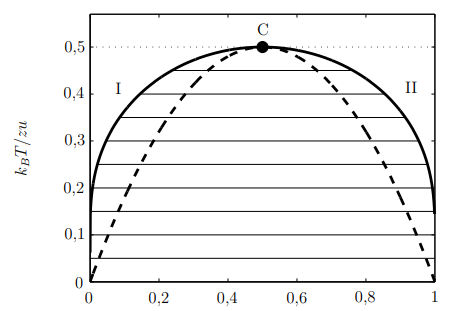
\includegraphics{../Fig/DiagrammePhaseMB}} \\
\textit{Diagramme de phases pour le modèle des solutions régulières avec $u > 0$. La courbe en pointillée est la spinodale, la courbe pleine est la courbe de coexistence liquide-liquide.}
\label{DPMB}
\end{center}
